\chapter{Display}

In diesem Kapitel gehen wir auf das Display ein, das im \textbf{Spiegel AI} Projekt verwendet wird. Wir beschreiben die Spezifikationen, die Installation und die Anpassungen, die vorgenommen wurden.

\section{Spezifikationen}
Beschreiben Sie die technischen Spezifikationen des Displays.

\section{Installation}
Erläutern Sie den Prozess der Installation des Displays.

\section{Anpassungen}
Beschreiben Sie etwaige Anpassungen oder Modifikationen am Display.

\subsection{eventuell HTMl seite und Aufbau oder in Installation}

\subsection{Widgets Aktualisierung}
Erarbeitet von: Leon Kranner \\ \\

Alle Widgets müssen in regelmäßiger Zeit aktualisiert werden. Wie regelmäßig dies der Fall ist, hängt vom Widget ab. Dies regelt die Timer.js Datei. Hier werden alle Widgets aktualisiert und die neusten Daten geladen. In diesem Abschnitt ist eine kleine Übersicht wie regelmäßig die Widgets geladen werden: \\

\begin{enumerate}
    \item \textbf{Uhr}
    Jede Sekunde
    
    \item \textbf{Termine:}
    Alle 60 Sekunden
    
    \item \textbf{JKalender:}
    Jeden Tag um Mitternacht
    
    \item \textbf{Wettervorhersage:}
    Alle 3 Stunden
    
    \item \textbf{Tankstellen:}
    Alle 10 Sekunden

 \item \textbf{Tankstellen:}
    Alle 10 Sekunden

 \item \textbf{Verkehrsinformationen:}
    Alle 5 Minuten
\end{enumerate}

\subsection{Termine Widget}
Erarbeitet von: Leon Kranner \\ \\

\noindent
Das Termin-Widget ist eine JavaScript-Anwendung, die dazu dient, die nächsten drei anstehenden Termine auf dem Display anzuzeigen. Dieses Widget filtert die Termine, sortiert sie nach Datum und stellt sicher, dass nur zukünftige Termine angezeigt werden. Die Termine werden dynamisch in eine HTML-Liste eingefügt. \\ \\
In Zukunft soll die App die nächsten Termine aus der Smartphone Kalender App abrufen und den Raspberry versenden. Somit werden die aktuellen Termine automatisch geladen und müssen nicht manuell eingetragen werden.

\begin{figure}[h]
    \centering
    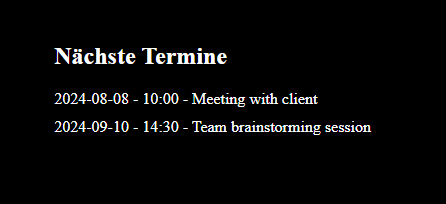
\includegraphics[width=0.4\textwidth]{pictures/appointments_widget.png}
  \captionsetup{justification=centering, labelformat=simple, singlelinecheck=false}
    \caption[Termine Widget]{Termine Widget\\ Quelle: eigene Darstellung}
\end{figure}

\noindent
Die Hauptfunktion des Widgets ist \texttt{loadAppointments()}, die beim Laden der Seite ausgeführt wird. Die Funktion filtert, sortiert und rendert die Termine auf dem Display.

\subsection*{Detaillierte Beschreibung der Funktion \texttt{loadAppointments}}
Die Funktion \texttt{loadAppointments()} führt folgende Schritte aus:

\begin{enumerate}
    \item \textbf{Terminliste initialisieren:}
    Ein Array von Terminen (\texttt{appointments}) wird definiert, das Datum, Uhrzeit und Beschreibung jedes Termins enthält.
    
    \item \textbf{Heutiges Datum ermitteln:}
    Das heutige Datum (\texttt{today}) wird mithilfe des \texttt{Date}-Objekts ermittelt.
    
    \item \textbf{HTML-Elemente vorbereiten:}
    Das HTML-Element mit der ID \texttt{appointmentsList} wird selektiert und dessen Inhalt wird geleert.
    
    \item \textbf{Filtern der zukünftigen Termine:}
    Es werden nur die Termine gefiltert, deren Datum gleich oder später als das heutige Datum ist.
    
    \item \textbf{Sortieren der Termine:}
    Die gefilterten Termine werden nach Datum sortiert.
    
    \item \textbf{Hinzufügen der Termine zur Liste:}
    Für jeden gefilterten und sortierten Termin wird ein \texttt{li}-Element erstellt, das die Termininformationen enthält. Diese \texttt{li}-Elemente werden zur \texttt{appointmentsList} hinzugefügt.
    
    \item \textbf{Seitenladezustand:}
    Die Funktion wird beim ersten mal in der appoinment.js Datei aufgerufen. Da sich Termine jederzeit ändern können, soll in regelmäßigen Abständen das Termin Widget aktualisiert werden.
\end{enumerate}

\noindent
Das Termin-Widget bietet eine einfache und effektive Lösung zur Anzeige bevorstehender Termine. Es lässt sich leicht in bestehende Webseiten integrieren und an individuelle Bedürfnisse anpassen.

\subsection{Kalender Widget}
Erarbeitet von Leon Kranner \\ \\

\noindent
Das Kalender-Widget ist eine JavaScript-Anwendung, die den aktuellen und den nächsten Monat in einem Kalender nebeneinander anzeigt. Der aktuelle Tag wird dabei hervorgehoben. \\

\begin{figure}[h]
    \centering
    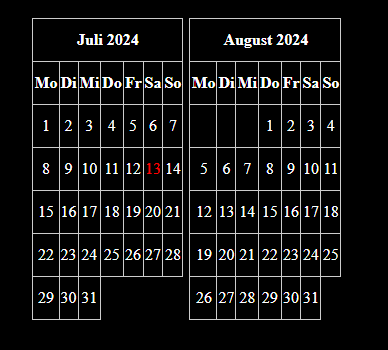
\includegraphics[width=0.5\textwidth]{pictures/calendar_widget.png}
  \captionsetup{justification=centering, labelformat=simple, singlelinecheck=false}
    \caption[Kalender Widget]{Kalender Widget\\ Quelle: eigene Darstellung}
\end{figure}

\noindent
Ursprünglich sollte der aktuelle Tag durch einen roten Ring markiert werden. Jedoch gab es Probleme bei der Formatierung, da die Zahl nicht mittig im Ring angezeigt wurde, sondern unübersichtlich an der Seite des Feldes., Gelöst wurde dieses Problem, in dem wir einen anderen Ansatz probiert haben. Der aktuelle Tag wird jetzt rot markiert und nicht eingekreist.\\
Ein weiteres Problem war die generelle Formatierung des Kalenders: Die Zahlen haben teilweise nicht mit den Wochentag übereingestimmt oder die Tage wurden leicht verschoben und haben nicht mehr gepasst. Außerdem hat der der erste Tag des Monats immer mit einen Montag begonnen. Nach einer längeren Bugfixing-Session und längerer Überarbeitung konnten die Fehler gelöst werden. \\
Zunächst wurden die Monate untereinander angezeigt. Da wir das Programm noch nicht auf dem Raspberry und den Bildschirm übertragen haben, konnten wir noch nicht testen, ob das Layout passt. Beim Testen viel auf, dass der zweite Monat abgeschnitten wurde, weshalb wir uns dazu entschieden haben, die Monate nebeneinander anzuzeigen.

\noindent
Die Hauptfunktion des Widgets ist \texttt{createCalendarWidget()}, die beim Laden der Seite ausgeführt wird. Diese Funktion generiert die Kalender für den aktuellen und den nächsten Monat und zeigt sie in definierten Containern nebeneinander an.

\subsection*{Detaillierte Beschreibung der Funktion \texttt{createCalendarWidget}}
Die Funktion \texttt{createCalendarWidget()} führt folgende Schritte aus:

\begin{enumerate}
    \item \textbf{Elemente vorbereiten:}
    \begin{itemize}
        \item Das HTML-Element mit der ID \texttt{calendarWidget} wird selektiert.
        \item Die HTML-Elemente für den aktuellen Monat (\texttt{currentMonthCalendar}) und den nächsten Monat (\texttt{nextMonthCalendar}) werden selektiert.
    \end{itemize}

    \item \textbf{Kalender generieren:}
    Die Funktion \texttt{generateCalendar()} wird verwendet, um den HTML-Code für die Kalender zu generieren und in die entsprechenden Container einzufügen.
    
    \item \textbf{Kalenderfunktion \texttt{generateCalendar()}:}
    \begin{itemize}
        \item Berechnung des ersten Tages des Monats und Anzahl der Tage im Monat.
        \item Aufbau des HTML-Codes für den Kalender mit den Monats- und Wochentagsnamen.
        \item Hinzufügen der Tage in die Tabelle, wobei der aktuelle Tag rot markiert wird.
    \end{itemize}

    \item \textbf{Anzeige des Kalenders:}
    Die Kalender für den aktuellen Monat und den nächsten Monat werden in den jeweiligen Containern angezeigt.

 \item \textbf{Seitenladezustand:}
    Die Funktion wird beim ersten mal in der Calendar.js Datei aufgerufen. Sollte sich das Profil bzw. der Zustand des Displays nicht ändern, wird jeden Tag um 24 Uhr der Kalender aktualisiert, um den nächsten Tag  bzw. den nächsten Monat anzeigen zu können.
\end{enumerate}

\noindent
Das Kalender-Widget bietet eine einfache und effektive Lösung zur Anzeige der aktuellen und kommenden Monatskalender. Es lässt sich leicht in den Smart Mirror integrieren und an individuelle Bedürfnisse anpassen. Die Hervorhebung des aktuellen Tages erleichtert die Orientierung im Kalender.


\subsection{Wettervorhersage Widget}
Erarbeitet von: Leon Kranner \\ \\

\noindent
Das Wettervorhersage-Widget ist eine JavaScript-Anwendung, die mithilfe der OpenWeatherMap API die Wettervorhersage für die nächsten drei Tage für eine bestimmte Stadt anzeigt. Das Widget lädt die Wetterdaten über eine API und zeigt die Vorhersage für den aktuellen Tag sowie die nächsten zwei Tage an. \\
In Zukunft soll man in der App den Standort auswählen können, damit der Nutzer entweder den Standort des Spiegels angeben kann oder z.B. auch das Wetter bei der OTH Regensburg ansehen können.

\begin{figure}[h]
    \centering
    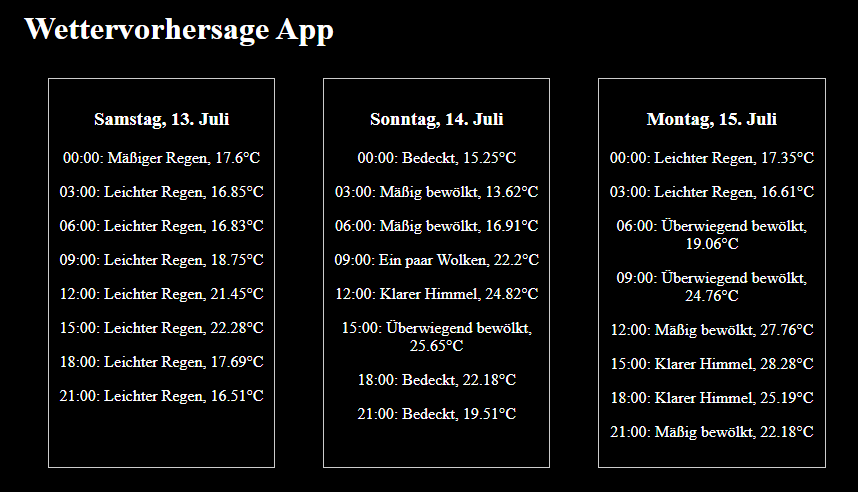
\includegraphics[width=0.4\textwidth]{pictures/forecast_widget.png}
  \captionsetup{justification=centering, labelformat=simple, singlelinecheck=false}
    \caption[Wettervorhersage Widget]{Wettervorhersage Widget\\ Quelle: eigene Darstellung}
\end{figure}

\noindent
Die Hauptfunktionen des Widgets sind \texttt{getForecast()} und \texttt{displayForecast(data)}. \texttt{getForecast()} ruft die Wetterdaten von der API ab, während \texttt{displayForecast(data)} die Daten verarbeitet und auf der Webseite anzeigt.

\subsection*{Detaillierte Beschreibung der Funktion \texttt{getForecast}}
Die Funktion \texttt{getForecast()} führt folgende Schritte aus:

\begin{enumerate}
    \item \textbf{API-Schlüssel und Stadt definieren:}
    Der API-Schlüssel und die Stadt, für die die Wettervorhersage abgerufen werden soll, werden definiert.
    
    \item \textbf{URL für den API-Aufruf erstellen:}
    Eine URL für den API-Aufruf wird mit dem API-Schlüssel und der Stadt erstellt.
    
    \item \textbf{API-Aufruf durchführen:}
    Ein Fetch-Aufruf wird durchgeführt, um die Wetterdaten von der OpenWeatherMap API abzurufen.
    
    \item \textbf{Fehlerbehandlung:}
    Falls die Stadt nicht gefunden wird oder ein anderer Fehler auftritt, wird eine Fehlermeldung angezeigt.
    
    \item \textbf{Daten verarbeiten:}
    Die erhaltenen Daten werden an die Funktion \texttt{displayForecast(data)} übergeben, um sie auf dem Display anzuzeigen.
\end{enumerate}

\subsection*{Detaillierte Beschreibung der Funktion \texttt{displayForecast(data)}}
Die Funktion \texttt{displayForecast(data)} führt folgende Schritte aus:

\begin{enumerate}
    \item \textbf{Vorhersage-Div vorbereiten:}
    Das HTML-Element mit der ID \texttt{forecast} wird selektiert und dessen Inhalt wird geleert.
    
    \item \textbf{Daten nach Tagen gruppieren:}
    Die Wetterdaten werden nach Tagen gruppiert und in einem Objekt gespeichert.
    
    \item \textbf{Vorhersage für drei Tage anzeigen:}
    Es werden nur die Vorhersagen für den aktuellen Tag und die nächsten zwei Tage angezeigt.
    
    \item \textbf{Tagesvorhersagen generieren:}
    Für jeden Tag wird ein Div-Element erstellt, das die Tagesvorhersage enthält. Jede Tagesvorhersage zeigt die Uhrzeit, eine Beschreibung des Wetters und die Temperatur an.
    
    \item \textbf{Vorhersagen in das HTML einfügen:}
    Die generierten Tagesvorhersagen werden in das HTML-Element \texttt{forecast} eingefügt.
\end{enumerate}


\noindent
Das Wettervorhersage-Widget bietet eine einfache und effektive Lösung zur Anzeige der Wettervorhersage für die nächsten drei Tage. Es lässt sich leicht im Display integrieren und an individuelle Bedürfnisse anpassen. Die Nutzung der OpenWeatherMap API ermöglicht eine zuverlässige und aktuelle Wettervorhersage.


\subsection{Notizen Widget}
Erarbeitet von: Leon Kranner \\ \\

\noindent
Das Notizen-Widget ist eine JavaScript-Anwendung, die es dem Benutzer ermöglicht, Notizen zu erstellen und zu speichern. Diese Notizen werden im lokalen Speicher des Browsers gespeichert, sodass sie auch nach dem Schließen des Browsers erhalten bleiben.

\begin{figure}[h]
    \centering
    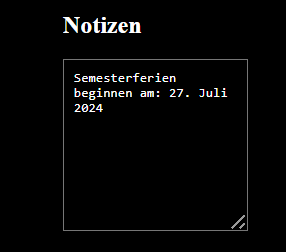
\includegraphics[width=0.4\textwidth]{pictures/notes_widget.png}
  \captionsetup{justification=centering, labelformat=simple, singlelinecheck=false}
    \caption[Notizen Widget]{Notizen Widget\\ Quelle: eigene Darstellung}
\end{figure}

\noindent
Die Hauptfunktionen des Widgets sind \texttt{loadNotes()} und \texttt{saveNotes()}. \texttt{loadNotes()} lädt die gespeicherten Notizen aus dem lokalen Speicher, während \texttt{saveNotes()} die Notizen im lokalen Speicher speichert.

\subsection*{Detaillierte Beschreibung der Funktion \texttt{loadNotes}}
Die Funktion \texttt{loadNotes()} führt folgende Schritte aus:

\begin{enumerate}
    \item \textbf{Gespeicherte Notizen abrufen:}
    Die Notizen werden aus dem lokalen Speicher des Browsers abgerufen.
    
    \item \textbf{Notizen im Textbereich anzeigen:}
    Wenn gespeicherte Notizen vorhanden sind, werden sie im Textbereich (\texttt{notesTextarea}) angezeigt.
\end{enumerate}

\subsection*{Detaillierte Beschreibung der Funktion \texttt{saveNotes}}
Die Funktion \texttt{saveNotes()} führt folgende Schritte aus:

\begin{enumerate}
    \item \textbf{Notizen aus dem Textbereich abrufen:}
    Der Inhalt des Textbereichs (\texttt{notesTextarea}) wird abgerufen.
    
    \item \textbf{Notizen im lokalen Speicher speichern:}
    Die Notizen werden im lokalen Speicher des Browsers gespeichert.
\end{enumerate}

\subsection*{Eventlistener}
Die Anwendung nutzt zwei Eventlistener:

\begin{itemize}
    \item \textbf{\texttt{DOMContentLoaded}-Event:}
    Lädt die Notizen, sobald die Seite vollständig geladen ist.
    
    \item \textbf{\texttt{input}-Event:}
    Speichert die Notizen, sobald der Benutzer den Text ändert.
\end{itemize}

\noindent
Das Notizen-Widget bietet eine einfache und effektive Lösung zur Erstellung und Speicherung von Notizen im lokalen Speicher des Browsers. Es lässt sich leicht in bestehende Webseiten integrieren und an individuelle Bedürfnisse anpassen. Die Nutzung des lokalen Speichers ermöglicht eine persistente Speicherung der Notizen, auch nach dem Schließen des Browsers.


\subsection{Uhr Widget}
Erarbeitet von: Marcel Wagner \\ \\
\noindent
Die Implementierung des Uhrzeit Widgets für den Smart Mirror ist ein wichtiger Schritt zur Verbesserung der Funktionalität und Benutzerfreundlichkeit des Geräts. Ziel dieses Widgets ist es, die aktuelle Uhrzeit exakt und zuverlässig anzuzeigen. Wobei die Anzeige in Echtzeit aktualisiert werden muss, um stets die genaue Uhrzeit widerzuspiegeln.\\ \\
Die Implementierung dieses Widgets basierte auf der Nutzung von JavaScript zur Echtzeitaktualisierung der Uhrzeit und HTML zur Einbettung des Widgets in die Benutzeroberfläche des Smart Mirrors. Desweiteren wurde CSS benutzt um das Widget zu formatieren. Die JavaScript Funktion sorgt dafür, dass die Uhrzeit jede Sekunde aktualisiert wird, während das HTML Dokument die Struktur definiert. Abschließend definiert die CSS Datei das Styling des Widgets. \\ \\
\noindent
Während der Entwicklung des Widgets traten mehrere Herausforderungen auf. Eine der größten Herausforderungen bestand darin, sicherzustellen, dass die Uhrzeit in Echtzeit und ohne Verzögerung aktualisiert wird. Dies war besonders wichtig, um die Genauigkeit der angezeigten Zeit zu gewährleisten. Die Verwendung der 'setTimeout' Funktion in JavaScript ermöglicht eine wiederholte Ausführung der Aktualisierungsfunktion in einem festgelegten Intervall von einer Sekunde, wodurch eine kontinuierliche und genaue Aktualisierung der Uhrzeit sichergestellt wurde.
Eine weitere Herausforderung war die exakte Zeitanzeige, insbesondere hierbei ist wichtig die Erwähnung der Formatierung der Uhrzeit, um sicherzustellen, dass Stunden, Minuten und Sekunden stets zweistellig angezeigt werden. Durch die Verwendung der 'padStart' Methode konnten die Zahlen auf eine konstante Länge von zwei Stellen gebracht werden, indem bei Bedarf führende Nullen hinzugefügt werden. Dies gewährleistete eine konsistente und gut lesbare Anzeige.\\ \\
\noindent
Die Implementierung des Uhrzeit Widgets verlief erfolgreich und erfüllt die gestellten Anforderungen. Die Uhrzeit wird zuverlässig und exakt in Echtzeit angezeigt. Das Widget integriert sich nahtlos in die Benutzeroberfläche des Smart Mirrors und bietet eine klare und gut lesbare Darstellung der aktuellen Uhrzeit.
Insgesamt stellt das Uhrzeit Widget eine wesentliche Funktionalität des Smart Mirrors dar. Der nachfolgenden Abbildung 1 kann das Implementierte Uhrzeit Widget auf der HTML Seite entnommen werden.

\begin{figure}[h]
    \centering
    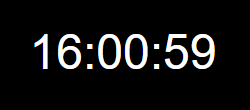
\includegraphics[width=0.4\textwidth]{pictures/time_widget.png}
  \captionsetup{justification=centering, labelformat=simple, singlelinecheck=false}
    \caption[Uhrzeit Widget]{Uhrzeit Widget\\ Quelle: eigene Darstellung}
\end{figure}

\subsection{Verkehrsinformation}
Erarbeitet von: Marcel Wagner \\ \\
\noindent
Die Implementierung des Stau-Widgets auf dem Smart Mirror stellt einen wichtigen Schritt dar, um den Nutzern eine umfassende und zuverlässige Quelle für aktuelle Verkehrsinformationen zur Verfügung zu stellen. Das Widget wurde speziell entwickelt, um eine Echtzeitübersicht über die Verkehrslage in Regensburg zu bieten, was insbesondere für Pendler und Reisende von großem Nutzen ist. Durch die Verwendung von JavaScript wurde eine nahtlose Integration mit der OpenStreetMap Overpass API realisiert, die als zuverlässige Datenquelle für Verkehrsdaten dient. \\ \\
\noindent
Die Strategie hinter der Implementierung war zweigleisig: Zum einen wurde eine sofortige Aktualisierung der Verkehrsinformationen beim Laden der Seite implementiert, um den Nutzern bei jedem Besuch des Smart Mirrors die aktuellsten Daten bereitzustellen. Zum anderen erfolgt eine regelmäßige automatische Aktualisierung alle fünf Minuten, um sicherzustellen, dass die angezeigten Informationen kontinuierlich aktuell gehalten werden. Dieser Ansatz gewährleistet eine hohe Aktualität und Relevanz der bereitgestellten Verkehrsinformationen. \\ \\
\noindent
Während der Entwicklung wurden mehrere Herausforderungen gemeistert, darunter die robuste Fehlerbehandlung, um sicherzustellen, dass Netzwerkprobleme oder API Ausfälle die Funktionalität des Widgets nicht beeinträchtigen. Ein besonderes Augenmerk lag auf der Gewährleistung einer stabilen und zuverlässigen Datenaktualisierung, die für eine nahtlose Benutzererfahrung entscheidend ist. \\ \\
\noindent
Das Verkehrs Widget präsentiert die Verkehrslage in einer klaren und intuitiven Benutzeroberfläche. Es informiert die Nutzer klar verständlich darüber, ob derzeit ein Stau vorliegt oder nicht, und bietet gegebenenfalls zusätzliche Informationen über Verkehrshindernisse oder Verkehrswarnungen. Diese klare visuelle Darstellung hilft den Nutzern, schnell zu erfassen, wie die aktuelle Verkehrssituation ihre geplante Route beeinflussen ist. \\ \\
\noindent
Insgesamt trägt das Verkehrs Widget erheblich zur Funktionalität und Benutzerfreundlichkeit des Smart Mirrors bei. Es bietet eine unverzichtbare Informationsquelle für die tägliche Routenplanung und unterstützt die Nutzer dabei, ihre Fahrtzeiten effizient zu optimieren. Das Implementierte Verkehrsinformationen Widget kann der nachfolgenden Abbildung entnommen werden. Diese Abbildung zeigt den Fall, dass aktuell gerade kein Stau  in den Straßen von Regensburg sind.

\begin{figure}[h]
    \centering
    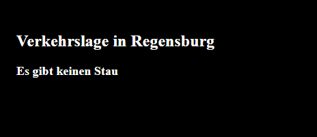
\includegraphics[width=0.4\textwidth]{pictures/traffic_widget.png}
  \captionsetup{justification=centering, labelformat=simple, singlelinecheck=false}
    \caption[Verkehrsinformations Widget]{Verkehrsinformations Widget\\ Quelle: eigene Darstellung}
\end{figure}

\subsection{Schlagzeilen}
Erarbeitet von: Marcel Wagner \\ \\
\noindent
Die Implementierung des Nachrichten Widgets für den Smart Mirror stellt einen wichtigen Schritt dar, um den Nutzern eine aktuelle und relevante Informationsquelle direkt auf seinem Smart Mirror zur Verfügung zu stellen. Das Widget wurde in JavaScript entwickelt und verwendet die 'RSS2JSON-API', um die neuesten Nachrichtenartikel eines ausgewählten RSS Feeds abzurufen und auf dem Smart Mirror anzuzeigen. Dies ermöglicht eine dynamische und automatische Aktualisierung der Nachrichteninhalte, sobald der Nutzer den Spiegel nutzt. \\ \\
\noindent
Ein zentrales Element der Implementierung ist die Verwendung des 'DOMContentLoaded' Events, das sicherstellt, dass das Widget erst aktiv wird, nachdem die gesamte Seite vollständig geladen ist. Dadurch wird sichergestellt, dass alle notwendigen Ressourcen und Elemente bereitstehen, bevor die Datenabfrage und die Darstellung der Nachrichten beginnen. \\ \\
\noindent
Die Funktionalität des Widgets umfasst die Asynchronität der Datenabfrage über die Fetch API, die die RSS Feeds von Nachrichtenquellen in ein JSON Format umwandelt, das vom JavaScript Code weiterverarbeitet werden kann. Dies ermöglicht eine schnelle und effiziente Bereitstellung der neuesten Nachrichteninhalte direkt auf dem Smart Mirror, ohne dass der Nutzer zusätzliche Schritte unternehmen muss, um sich auf dem Laufenden zu halten. \\ \\
\noindent
Eine besondere Herausforderung während der Implementierung war die unterschiedliche Verfügbarkeit von RSS Feeds bei verschiedenen Nachrichtenseiten. Viele führende Nachrichtenagenturen und Zeitungen bieten zwar RSS Feeds an, einige jedoch nicht oder beschränken den Zugang zu ihren Inhalten über diese Schnittstelle. Dies erforderte eine sorgfältige Auswahl geeigneter RSS Feeds, die eine kontinuierliche und zuverlässige Datenversorgung gewährleisten konnten. Die Ausgegeben Nachrichten dieses Widget entspannen der Frankfurter Allgemeinen Zeitung \\ \\
\noindent
Um die Benutzerfreundlichkeit zu maximieren, wurde die Benutzeroberfläche des Widgets bewusst einfach und intuitiv gestaltet. Die angezeigten Nachrichten werden in einer geordneten Liste präsentiert. \\ \\
\noindent
Zusammenfassend bietet das Nachrichten Widget einen bedeutenden Mehrwert für den Smart Mirror, indem es den Nutzern eine einfache und effektive Möglichkeit bietet, sich über aktuelle Ereignisse zu informieren. Die Implementierung war erfolgreich in Bezug auf die gesetzten Ziele. Der Nachfolgenden Abbildung kann das implementierte Widget auf dem Smart Mirror entnommen werden.

\begin{figure}[h]
    \centering
    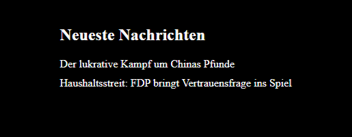
\includegraphics[width=0.4\textwidth]{pictures/news_widget.png}
  \captionsetup{justification=centering, labelformat=simple, singlelinecheck=false}
    \caption[News Widget]{News Widget\\ Quelle: eigene Darstellung}
\end{figure}

\subsection{Tankstellen}
Erarbeitet von: Marcel Wagner \\ \\
\noindent
Die Implementierung des Tankstellen Widgets für den Smart Mirror verfolgt das Ziel, den Nutzern eine praktische und zeitnahe Information über den günstigsten Kraftstoffpreise einer Tankstelle in der Nähe zu bieten. Diese Funktionalität wurde durch die Integration von JavaScript und die Nutzung der Tankerkoenig API realisiert, die speziell auf die Abfrage von Tankstellenpreisen und Tankstelleninformationen ausgerichtet ist. \\ \\
\noindent
Zu Beginn des Implementierungsprozesses wird der 'DOMContentLoaded' Eventlistener verwendet, um sicherzustellen, dass sämtliche Inhalte der Webseite geladen sind, bevor die Datenabfrage gestartet wird. Dies gewährleistet eine stabile und zuverlässige Performance des Widgets auf dem Smart Mirror. Die API Anfrage erfolgt unter Verwendung eines spezifischen API Schlüssels, der die Authentifizierung gegenüber der Tankerkoenig API ermöglicht. Der Standortbezug erfolgt für die Stadt Regensburg mit definierten geografischen Koordinaten und einem Suchradius von 5 Kilometern, um die Tankstellen in unmittelbarer Umgebung zu erfassen. \\ \\
\noindent
Die Datenabfrage wird asynchron durchgeführt, um eine reibungslose Interaktion mit der API zu gewährleisten. Nachdem die Daten abgerufen wurden, erfolgt eine Überprüfung auf erfolgreiche Antwort und die Verfügbarkeit von Tankstelleninformationen. Falls die API Daten erfolgreich zurückgegeben werden und Tankstelleninformationen vorhanden sind, wird die günstigste Tankstelle ermittelt. Dies geschieht durch einen Vergleich der Kraftstoffpreise der abgerufenen Tankstellen, wobei die preisgünstigste Option ausgewählt und deren Informationen weiterverarbeitet werden. \\ \\
\noindent
Ein zentraler Aspekt der Implementierung ist die robuste Fehlerbehandlung, die sicherstellt, dass der Nutzer bei Problemen wie Netzwerkfehlern oder unerwarteten API Antworten angemessen informiert wird.  \\ \\
\noindent
Die Darstellung der Tankstelleninformationen auf dem Smart Mirror erfolgt in einer klar strukturierten Form. Dies umfasst den Namen der Tankstelle, die vollständige Adresse inklusive Straße, Hausnummer, Postleitzahl und Ort sowie den aktuellen Preis pro Liter Kraftstoff. Diese Informationen sind leicht zugänglich und ermöglichen es dem Nutzer, schnell die wichtigsten Details zu erfassen und eine informierte Entscheidung zu treffen. \\ \\
\noindent
Die Implementierung des Tankstellen Widgets erweitert somit die Funktionalität des Smart Mirrors erheblich, indem sie eine praktische Lösung für die Überwachung und Optimierung der Kraftstoffkosten bietet.

\begin{figure}[h]
    \centering
    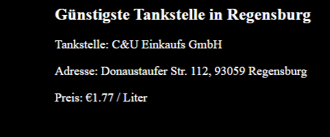
\includegraphics[width=0.4\textwidth]{pictures/gasstation_widget.png}
  \captionsetup{justification=centering, labelformat=simple, singlelinecheck=false}
    \caption[Tankstellen Widget]{Tankstellen Widget\\ Quelle: eigene Darstellung}
\end{figure}

\subsection{Test Verfahren}
Erarbeitet von: Leon Kranner und Marcel Wagner \\ \\
\noindent
Für die implementierten Widgets auf dem Smart Mirror wurden umfangreiche Testverfahren angewendet, die sowohl die Funktionalität als auch die Benutzererfahrung der einzelnen Widgets sicherstellen sollen. Diese unterschiedlichen Testverfahren werden nun im Folgenden genauer beschrieben. \\ \\
\noindent
\textbf{Funktionalitätstests:} Dieser Test konzentrierten sich auf die grundlegenden Aufgaben jedes Widgets. Das Uhrzeitwidget wurde auf seine Fähigkeit getestet, die aktuelle Uhrzeit präzise anzuzeigen. Außerdem wurde sichergestellt, dass die Darstellung formatiert und korrekt aktualisiert wird. Beim News Widget lag der Fokus auf der korrekten Abrufung und Darstellung aktueller Nachrichten, wobei sichergestellt wurde, dass die Informationen stets aktuell und relevant sind. Das Tankstellenwidget durchlief API Integrationstests, um sicherzustellen, dass die Kraftstoffpreise korrekt von der Tankerkoenig API abgerufen und in einem klaren Format angezeigt werden. Das Verkehrsinformations Widget wurde auf seine Fähigkeit geprüft, Verkehrsinformationen zeitnah abzurufen und zuverlässig darzustellen, um Nutzer vor aktuellen Verkehrsbehinderungen zu warnen. \\ \\
\noindent
\textbf{Benutzererfahrungstests:} Diese waren entscheidend, um sicherzustellen, dass die Widgets intuitiv sind. Hierbei halfen Usability Tests, diese bewerteten die Widgets auf Benutzerfreundlichkeit der Benutzeroberfläche. Dabei wurde besonders darauf geachtet, dass die Widgets übersichtlich gestaltet sind und Nutzer schnell die benötigten Informationen finden können. \\ \\
\noindent
\textbf{Performance- und Lasttests:} Diese Testverfahren waren ebenfalls Teil der Teststrategie, um sicherzustellen, dass die Widgets unter verschiedenen Bedingungen effizient arbeiten. Ladezeittests wurden durchgeführt, um sicherzustellen, dass die Widgets schnell genug reagieren und Daten effizient verarbeiten. Skalierbarkeitstests wurden genutzt, um sicherzustellen, dass die Widgets auch bei erhöhtem Datenverkehr stabil bleiben und keine übermäßigen Ressourcen verbrauchen, was besonders wichtig für die Langzeitnutzung ist. \\ \\
\noindent
\textbf{Integrationstest:} Dabei wurden Kompatibilitätstests durchgeführt, um sicherzustellen, dass die Widgets reibungslos mit anderen Komponenten des Smart Mirrors interagieren. Systemtests prüften die Gesamtfunktionalität des Smart Mirrors unter verschiedenen Betriebsbedingungen, um sicherzustellen, dass alle Widgets harmonisch zusammenarbeiten und die Gesamtleistung des Systems nicht beeinträchtigen werden. \\ \\
\noindent
Diese umfassenden Testverfahren stellen sicher, dass die implementierten Widgets nicht nur funktional sind, sondern auch eine qualitativ hochwertige Benutzererfahrung bieten und unter allen Bedingungen zuverlässig arbeiten.



